\section{Physics at Hadron Colliders}

The LHC collides protons together in order to create collisions with center of mass energy \sqrts.
During a collision, the constituents of the protons may interact directly and exchange a substantial fraction of their proton's momentum, in a process called hard-scattering.
These interactions may be quark-quark, quark-gluon, or gluon-gluon scattering events that can be described with a degree of fidelity by a matrix element complication.
This is a messy process, and is complicated by the composite nature of the protons.
This section describes the basis of how colliding protons may produce the types of events that are of interest for this thesis.

\subsection{Parton distribution function}

\begin{figure}[h!]
\captionsetup[subfigure]{position=b}
\centering
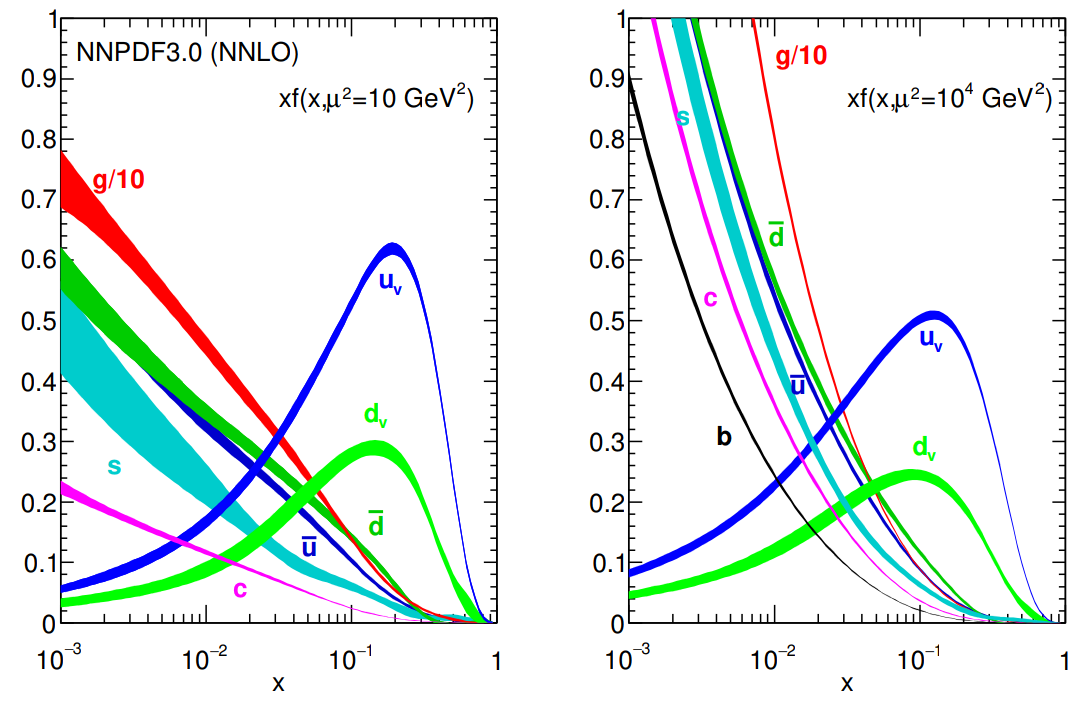
\includegraphics[width=0.99\textwidth]{figures/pheno/pdgpdf.png}
\caption{Parton distribution functions $xf_i(x,Q)$ calculated using NNPDF3.0 with energy scale $Q^2=10\text{~GeV}^2$ (left) and $Q^2=10^4\text{~GeV}^2$ (right). This figure is from \ref{Ball:2014uwa}.}
\label{fig:partDistFunc}
\end{figure}

The protons that make up the colliding beams at the LHC are bound states of quarks and gluons, collectively called partons.
These consist of three valance quarks ($uud$), and a \emph{sea} or virtual quark/anti-quark pairs.
When two protons collide with sufficient energy \footnote{On the scale of $\Lambda_\text{QCD}\approx218$~MeV.}, two types of qualitative processes take place.
First is \emph{hard-scattering}, an interaction mediated by a large momentum exchange between typically two partons.
Second is \emph{soft-scattering}, where the remaining partons interact through the low energy mediators.
While both processes are interesting, hard interactions are of particular interest in this thesis, as these provide access to particularly high energy interactions.

When two partons interact each carries a fraction of their respective proton's total energy \sqrts.
The longitudinal component of the momentum fraction is termed Feynman's $x$.
When a high energy probe particle collides with a proton, the probe will hard-scatter off of one of the proton's constituents be it a quark or gluon.
In $pp$ collisions, the probe is a parton selected from a proton in the opposing beam.
The of the probe probability to scatter of a particular parton $i$ depends on both its momentum fraction $x$ and the momentum exchange $Q$.
This differential probability function, $f_i(x,Q)$, is called the parton distribution function (PDF).
Hence, $f_u(x,Q)$ gives the that the probe will interact with an up quark, while $f_{\overline{s}}(x,Q)$ gives the corresponding probability for an interaction with an anti-strange quark.

The dynamics within the proton that determine PDFs take place at low $Q$, where calculations are complicated by the large QCD coupling from Equation \ref{eqn:alphas}.
Instead of analytic calculations, PDFs functions are fit to experimental measurements.
The resulting PDF shapes as a function of $x$ is shown in Figure \ref{fig:partDistFunc} for each parton.
The valance quark ($u$ and $d$) are seen to have peaks between $x=0.1$ and $x=0.2$, indicating a relatively high frequency that these carry a large portion of the proton's momentum.
In contrast, the sea quarks ($\overline{u}$, $\overline{d}$, $s/\overline{s}$, and $c/\overline{c}$) typically carry a much smaller momentum fraction.
The $u$ and $d$ quarks contribute to the sea as well, and Figure \ref{fig:partDistFunc} actually separates out the valance component from the sea component for these.
The PDFs of the sea $u$ and $d$ quarks and anti-quarks are identical since these are produced in virtual pairs.
The PDFs for gluons are shown scaled down by a factor of 10, as nearly half the proton's momentum is carried by gluons.\cite{wells}

The differential cross sections of an $2\to X$ interaction, given in Equation \ref{eqn:diffCrossSection}, depend on the initial state particles.
When two protons collide, the initial state particles of a hard-scattering process are selected randomly from each proton according to the parton distribution functions.
Consequently the total cross section of a $pp$ collision corresponds to a sum over partons $i,j$ in each proton respectively, and an integral over momentum fractions.
The $pp$ version of the differential cross section is given in Equation \ref{eqn:ppDiffCrossSection}.
\begin{equation}\begin{split}\label{eqn:ppDiffCrossSection}
d\sigma(pp\to X)=\sum_i\sum_j\int_0^1dx_i\int_0^1dx_j~d\sigma(ij\to X)f_i(x_i)f_j(x_j)
\end{split}\end{equation} 
This sum tallies the cross sections $d\sigma(ij\to X)$ for each possible configuration of initial states, weighted by the likelihood of the initial state $ij$.

\subsection{Parton Luminosity}

\begin{figure}[h!]
\captionsetup[subfigure]{position=b}
\centering
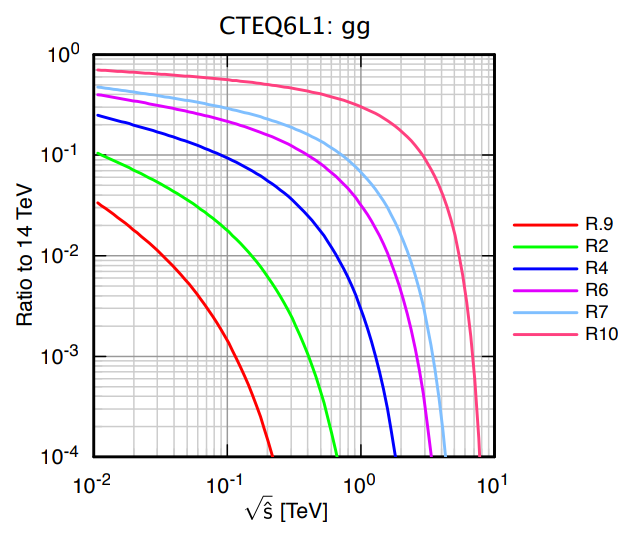
\includegraphics[width=0.5\textwidth]{figures/pheno/partonLumi.png}
\caption{Comparison of $gg$ luminosity for different \sqrts, plotted as a ratio to the luminosity at \sqrts=14~TeV. Figure from \cite{quigg}.}
\label{fig:partonLumi}
\end{figure}

The luminosity defined in Equation \ref{eqn:lumi} is defined in terms of the $pp$ cross section $\sigma_{pp}$.
A more specific \emph{parton luminosity} $\mathcal{L}_{ij}$ may be defined for particular species of parton $i$ and $j$ with center of mass energy $\sqrths<\sqrts$.
The ``hatted'' variables correspond to values in the parton's center of mass frame.
\begin{equation}\begin{split}\label{eqn:partonLumi}
\frac{\tau}{\shat}\frac{d\mathcal{L}_{ij}}{d\tau}\equiv\frac{\tau}{\shat(1+\delta_{ij})} \int_\tau^1 \frac{dx}{x}~f_i(x)f_j(\tau/x)+f_j(x)f_i(\tau/x)]
\end{split}\end{equation}
This definition supposes the beam consists of partons rather than protons, and each parton combination has an associated luminosity that is a function of the fraction $\tau=\shat/s$.
This luminosity is seen to depend on the beam energy through the presence of the PDFs and Feynman's $x$.
The total cross section for $pp\to X$ is defined by with a sum over parton species,
\begin{equation}\begin{split}
\sigma_{pp\to X}(s)=\sum_i\sum_j \frac{d\tau}{\tau}\cdot\frac{\tau}{\shat}\frac{d\mathcal{L}_{ij}}{d\tau}\cdot[\shat\sigma_{ij\to X}(\shat)].
\end{split}\end{equation} 
As indicated by the shapes of PDF curves, the parton luminosity for a beam of energy \sqrts drops off as a function of \sqrths.
\cite{quigg}

As a consequence, although the LHC collides beams with \sqrts=13~TeV, the practical luminosity of collisions with \sqrths=13~TeV essentially vanishes.
This limits the energy available in hard scattering to a fraction of \sqrts.
For example, the invariant-mass of the most energetic two-jet event recorded by ATLAS in Run~2 is just $m_{jj}=8$~TeV.
A second consequence of Equation \ref{eqn:partonLumi} arises from its dependence on the proton center of mass energy \sqrts (through $\tau$).
Increasing the \sqrts greatly expands the parton luminosity at large \sqrths.
Both of these effects are illustrated in Figure \ref{fig:partonLumi}, which plots the ratio of $gg$ parton luminosities at different center of mass energies to the LHC design value.

\section{Standard Model Dilepton Production}\label{sec:phenoBkg}

Both the \hmm search and the non-resonant search share a similar interest in the dilepton invariant mass spectra.
As such the backgrounds for these analyses share a similar composition produced by standard model processes.
The dominant hard-scattering processes that produce events with dilepton pairs in the high invariant-mass region at the LHC are described in this section.

\begin{figure}[h!]
\captionsetup[subfigure]{position=b}
\centering
    \feynmandiagram [medium,baseline=(v1.base),horizontal=v1 to v2] {
    q1[particle=\(q\)] --[fermion] v1 --[boson,edge label=\(\gamma^*/Z\)] v2 --[fermion] z1[particle=\(\ell^-\)],
    v1 --[fermion] q2[particle=\(\overline{q}\)],
    z2[particle=\(\ell^+\)] --[fermion]v2,
    }; \\ [1em]
\caption{Feynman diagram for the leading order Drell-Yan process.}
\label{fig:phenoDy}
\end{figure}

The most significant lepton pair production mechanism in hadronic collisions was proposed in 1970 Sidney Drell and Tung-Mow Yan. 
The process is described as the annihilation of partons from opposing protons in order to produce a massive intermediate state that carries the momentum exchange of the collision. \cite{drellYan}
For collision energies below the \Z mass, this intermediate state is an off-shell photon.
Above the \Z mass, both photons and \Z bosons mediate Drell-Yan production as illustrated in Figure \ref{fig:phenoDy}.
The predicted differential cross section falls sharply as the produced dilepton pair's invariant mass grows.
Although this prediction is inaccurate near the \Z mass where resonant production dominates, in the kinematic regions of interest for this thesis it describes the background to first order.

\begin{figure}[h!]
\captionsetup[subfigure]{position=b}
\centering
\subfloat[][]{{
    \feynmandiagram [medium,baseline=(v1.base),vertical=v2 to v1] {
    b[particle=\(q\)] --[fermion] v2,
    v2 --[boson] t[particle=\(Z\)],
    v1 --[boson] qb[particle=\(Z\)],
    v1 --[fermion] qa[particle=\(\overline{q}'\)],
    v2 --[fermion] v1,
    };
}}
\hspace{2em}
\subfloat[][]{{
    \feynmandiagram [medium,baseline=(v1.base),horizontal=v1 to v2] {
    q1[particle=\(q\)] --[fermion] v1 --[boson,edge label=\(W\)] v2 --[boson] z1[particle=\(Z\)],
    v1 --[fermion] q2[particle=\(\overline{q}'\)],
    v2 --[boson] z2[particle=\(W\)],
    };
}}
\subfloat[][]{{
    \feynmandiagram [medium,baseline=(v1.base),horizontal=v1 to v2] {
    q1[particle=\(q\)] --[fermion] v1 --[boson,edge label=\(Z\)] v2 --[boson] z1[particle=\(W^-\)],
    v1 --[fermion] q2[particle=\(\overline{q}\)],
    v2 --[boson] z2[particle=\(W^+\)],
    };
}}
\caption{Representative Feynman diagrams for leading order diboson production for ZZ (a) WZ (b) and WW (c). \check}
\label{fig:phenoDibosn}
\end{figure}

The next leading source of dilepton events come from \emph{diboson} production.
These described by diagrams, including those in Figure \ref{fig:phenoDibosn}, with two vector bosons \W or \Z in their final state.
The leading order production of these events is through the $q\qbar$ initial state.

\begin{figure}[h!]
\captionsetup[subfigure]{position=b}
\centering
\subfloat[][]{{
    \feynmandiagram [medium,baseline=(v1.base),horizontal=v1 to v2] {
    b[particle=\(g\)] --[gluon] v1  --[gluon] v2,
    v2 --[fermion] t[particle=\(t\)],
    qa[particle=\(g\)]--[gluon]v1,
    qb[particle=\(\overline{t}\)]--[fermion]v2,
    };
}}
\hspace{2em}
\subfloat[][]{{
    \feynmandiagram [medium,baseline=(v1.base),vertical=v1 to v2] {
    g1[particle=\(g\)] --[gluon] v1,
    t1[particle=\(\overline{t}\)] --[fermion]v1,
    g2[particle=\(g\)] --[gluon] v2 --[fermion] t2[particle=\(t\)],
    v1 --[fermion] v2,
    };
}}
\hspace{2em}
\subfloat[][]{{
    \feynmandiagram [medium,baseline=(v1.base),horizontal=v1 to v2] {
    b[particle=\(q\)] --[fermion] v1  --[gluon] v2,
    v2 --[fermion] t[particle=\(t\)],
    v1--[fermion]qa[particle=\(\overline{q}\)],
    qb[particle=\(\overline{t}\)]--[fermion]v2,
    };
}}
\caption{Representative Feynman diagrams for leading order $t\tbar$ production.}
\label{fig:phenoTtbar}
\end{figure}

\begin{figure}[h!]
\captionsetup[subfigure]{position=b}
\centering
\subfloat[][]{{
    \feynmandiagram [small,baseline=(v1.base),horizontal=qa to qb] {b[particle=\(q\)] --[fermion] v2 --[fermion] t[particle=\(q'\)],qa[particle=\(b\)] --[fermion] v1 --[fermion] qb[particle=\(t\)],v2 --[boson] v1};
}}
\hspace{2em}
\subfloat[][]{{
    \feynmandiagram [small,baseline=(v1.base),horizontal=v1 to v2] {
    b[particle=\(q\)] --[fermion] v1  --[boson,edge label=\(W\)] v2,
    v2 --[fermion] t[particle=\(t\)],
    v1--[fermion]qa[particle=\(\overline{q}'\)],
    qb[particle=\(\overline{b}\)]--[fermion]v2,
    };
}}
\hspace{2em}
\subfloat[][]{{
    \feynmandiagram [small,baseline=(v1.base),horizontal=v1 to v2] {
    b[particle=\(g\)] --[gluon] v1  --[fermion] v2,
    v2 --[fermion] t[particle=\(t\)],
    qa[particle=\(b\)]--[fermion]v1,
    qb[particle=\(W\)]--[boson]v2,
    };
}}
\hspace{2em}
\subfloat[][]{{
    \feynmandiagram [small,baseline=(v1.base),vertical=v1 to v2] {
    b[particle=\(b\)] --[fermion] v1 --[boson] w[particle=\(W\)],
    g[particle=\(g\)] --[gluon] v2 --[fermion] t[particle=\(t\)],
    v1 --[fermion] v2,
    };
}}
\caption{Representative Feynman diagrams for leading order single-top production. Subfigures (a) and (b) show $s$-channel and $t$-channel diagrams respectively. Subfigures (c) and (d) show the leading order $bg\to Wt$ diagrams.}
\label{fig:phenoSingleTop}
\end{figure}

Figure \ref{fig:phenoTtbar} lists diagrams for the production of pairs of top quarks: $t\tbar$.
The leading order diagrams produce top quarks through interactions with gluons.
Figure \ref{fig:phenoSingleTop} shows diagrams for single-top production.
This primarily takes place through production with a lighter quark.
At the LHC, the $t$-channel production shown in Figure \ref{fig:phenoSingleTop} (b) is most prevalent, since the $s$-channel diagram requires a bottom quark initial state. \cite{Kidonakis:2011wy}
Additional production exists in conjunction with a \W boson, which also requires an initial state bottom quark. \cite{Kidonakis:2010ux}
After being produced, the top quarks rapidly decay to a \W and lighter quark (bottom, strange, or down) final state.
Most ($96\pm3\%$) top quarks decay to a final state with a bottom quark. \cite{pdg2018}
The result is, in some cases, a final state with multiple leptons.

\cite{Kidonakis:2011wy, Kidonakis:2010ux}



% \afterpage{
% \begin{table}[htp]
% \begin{center}
% \begin{tabular}{C{0.3\textwidth} C{0.5\textwidth}}
% \toprule
% Process & Diagram \\
% \midrule
% Drell-Yan & 
%     \feynmandiagram [medium,baseline=(v1.base),horizontal=v1 to v2] {
%     q1[particle=\(q\)] --[fermion] v1 --[boson,edge label=\(\gamma^*/Z\)] v2 --[fermion] z1[particle=\(\ell^-\)],
%     v1 --[fermion] q2[particle=\(\overline{q}\)],
%     z2[particle=\(\ell^+\)] --[fermion]v2,
%     }; \\ [1em]
% Diboson &
%     \feynmandiagram [medium,baseline=(v1.base),horizontal=v1 to v2] {
%     q1[particle=\(q\)] --[fermion] v1 --[boson] v2 --[boson] z1[],
%     v1 --[fermion] q2[particle=\(\overline{q}'\)],
%     v2 --[boson] z2[],
%     }; \\ [1em]
% Single-top & 
%     \feynmandiagram [medium,baseline=(v1.base),horizontal=v1 to v2] {
%     b[particle=\(q\)] --[fermion] v1  --[boson,edge label=\(W\)] v2,
%     v2 --[fermion] t[particle=\(\overline{t}\)],
%     v1--[fermion]qa[particle=\(\overline{q}'\)],
%     qb[particle=\(b\)]--[fermion]v2,
%     }; \\ [1em]
% Wt & 
%     \feynmandiagram [medium,baseline=(v1.base),horizontal=v1 to v2] {
%     b[particle=\(g\)] --[gluon] v1  --[fermion] v2,
%     v2 --[fermion] t[particle=\(t\)],
%     qa[particle=\(b\)]--[fermion]v1,
%     qb[particle=\(W\)]--[boson]v2,
%     }; \\ [1em]
% $t\tbar$ &
%     \feynmandiagram [medium,baseline=(v1.base),horizontal=v1 to v2] {
%     b[particle=\(g\)] --[gluon] v1  --[gluon] v2,
%     v2 --[fermion] t[particle=\(t\)],
%     qa[particle=\(b\)]--[gluon]v1,
%     qb[particle=\(t\)]--[fermion]v2,
%     }; \\
% \bottomrule
% \end{tabular}
% \caption{Representative Feynman diagrams for the leading background processes for dilepton events at the LHC. In several cases additional diagrams contribute at leading order. These will be specified in more detail in the context in which they are relevant.}
% \label{tab:phenoBkg}
% \end{center}
% \end{table}
% \clearpage
% }

\section{Higgs Production Mechanisms}\label{sec:phenoHiggs}

\begin{figure}[h!]
\captionsetup[subfigure]{position=b}
\centering
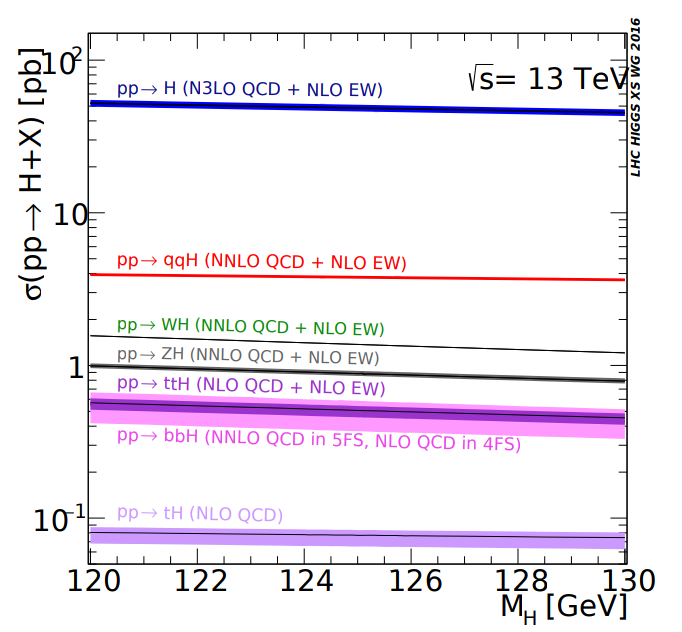
\includegraphics[width=0.5\textwidth]{figures/pheno/higgsXsec.png}
\caption{The cross sections of various higgs production mechanisms shown as a function of Higgs mass. {\color{red} address different names in plot} \cite{higgsCross}}
\label{fig:higgsCrossSection}
\end{figure}

The total production cross section for Higgs bosons at the LHC is 54.7~pb at N3LO precision \cite{higgsCross}.
Higgs bosons are produced through several distinct mechanisms at the LHC.
These are distinguished by both their initial states and the topology of their final states.
The leading production, responsible for 89\% of all Higgs, is through gluon-gluon fusion (ggF).
Although there is no direct coupling between gluons and the Higgs, the interaction is mediated by a heavy quark loop.
The next leading production is vector boson fusion (VBF) with roughly 9\% the cross section as ggF.
In this process, the Higgs is produced through a ``collision'' of either \W or \Z bosons.
The final state includes the Higgs, along with two quarks that rapidly patronize to form jets.
The presence of two jets in the final state help distinguish VBF events from background processes, and ameliorates the challenge of its low cross section.
The weakest production mechanisms are ttH and bbH, where the Higgs is produced in conjunction with a top or bottom quark pair.

The production mechanisms with the third largest cross section are collectively called ``Higgs produced in association with a vector boson'', or VH.
These are the primary focus for the \hmm search presented in this thesis.
There are several ``sub-mechanisms'' that contribute to VH.
Of these, the one with the largest cross section is the s-channel production with initial state quarks whimsically called \emph{Higgsstrahlung} in analogy to Bremsstrahlung radiation.
When the mediator boson is a \W, then Higgsstrahlung is responsible for the leading order WH production mechanism.
As a result of the corresponding parton luminosities, the cross section of WH depends on the sign of the mediating $W$ boson: the production positively charged \Wp benefits from the enhanced PDF of valance $u$-quarks seen in Figure \ref{fig:partonLumi}. \check
The cross section for WH is given in Equation \ref{eqn:whxs}.

\begin{equation}\begin{split}\label{eqn:whxs}
\sigma(q_i\qbar_j\to WH)=\frac{\pi\alpha^2 |V_{ij}|^2}{36 \sin^4\theta_W} \frac{2k}{\sqrts} \frac{k^2+3m^2_W}{(s-m^2_W)^2}
\end{split}\end{equation} 
Here $V_{ij}$ are the CKM matrix elements, $k$ is the center of mass momentum of the Higgs, and $\theta_W$ is the Weinberg angle defined in Section \ref{sec:ewTheory}.

When the mediator boson is a \Z, then Higgsstrahlung is the leading production mechanism for ZH as well.
The cross section for ZH in $pp$ collisions is given in Equation \ref{eqn:zhxs}.
\begin{equation}\begin{split}\label{eqn:zhxs}
\sigma(f\overline{f}\to ZH)=\frac{\pi\alpha^2 \ell_f^2r_f^2}{48N_c\sin^4\theta_W\cos^4\theta_W} \frac{2k}{\sqrts} \frac{k^2+3m^2_Z}{(s-m^2_Z)^2}
\end{split}\end{equation} 
Here, $r\equiv-2Qx_W$, $\ell\equiv2(T_3-Qx_W$,
$T_3$ is the third component of weak isospin for the left-handed $f$, $Q$ is its electric charge, and $x_W\equiv\sin^2\theta_W$.
While Equation \ref{eqn:zhxs} describes the $q\qbar\to ZH$ cross section, it is also applicable to $\ell^+\ell^-$ collisions that might take place in future lepton colliders.
This makes this process of particular interest for precision measurements of Higgs properties.

Unlike with WH, the sub-leading mechanisms are not negligible for ZH.
These consist of interactions with two initial state gluons where the Higgs is produced via a heavy quark loop.
There are two diagrams to consider, one a ``box'' diagram, and one a ``triangle'' diagram.
Together, these represent $\approx10\%$ of the total ZH cross section.

\begin{table}[htp]
\begin{center}
{\footnotesize
\begin{tabular}{l | l | l l l}
\toprule
Production & Cross section [pb] & Uncertainty (theory) [\%] & Uncertainty (PDF/$\alpha_s$) [\%] \\
\midrule
Gluon-gluon fusion (ggF)  & 48.58       & +4.56, -6.27 & $\pm3.20$  \\
Vector boson fusion (VBF) &  4.28       & +0.5, -0.3 & $\pm2.1$  \\
Associated W (WH)         & 1.513       & +0.4, -0.7 & $\pm1.8$  \\
$\hookrightarrow$  $\Wp\to\ell^+\nu$    &$\hookrightarrow$ 0.10363 &$\hookrightarrow$ +0.3, -0.8 &$\hookrightarrow$ $\pm1.8$  \\
$\hookrightarrow$  $\Wm\to\ell^-\nu$    &$\hookrightarrow$ 0.6649  &$\hookrightarrow$ +0.5, -0.6 &$\hookrightarrow$ $\pm1.9$  \\
Associated Z (ZH)         & 0.9861      & +3.8, -3.3 & $\pm1.6$  \\
$\hookrightarrow$  $Z\to\ell^+\ell^-$   &$\hookrightarrow$ 0.03327 &$\hookrightarrow$ +3.8, -3.3 &$\hookrightarrow$ $\pm1.6$  \\
ttH                       &  0.6137     & +6.0, -9.2 & $\pm3.5$  \\
\bottomrule
\end{tabular}
}
\caption{Vector boson leptonic decays include $\tau$. Higgs mass at 125 GeV.\cite{higgsCross}}
\label{tab:higgsCrossSec}
\end{center}
\end{table}

The diagrams for VH processes, along with the other leading production mechanisms, are shown in Table \ref{tab:higgsProdDiagrams}.
The cross sections and the associated theoretical uncertainties, are given in Table \ref{tab:higgsCrossSec}.
As mentioned earlier, these cross sections depend on the Higgs mass. The Numbers in Table \ref{tab:higgsCrossSec} are calculated with \mh=125~GeV, and the functional dependence is shown in Figure \ref{fig:higgsCrossSection}.

\begin{table}[p!]
\begin{center}
{\footnotesize
\begin{tabular}{C{0.3\textwidth} C{0.5\textwidth}}
\toprule
Higgs Production & Diagram \\
\midrule
\centered{Gluon-gluon fusion}  &
\centered{\begin{tikzpicture}
\begin{feynman}
    \vertex (h){\(H\)};
    \vertex [left=of h] (v);
    \vertex [above left=of v] (p1);
    \vertex [below left=of v] (p2);
    \vertex [left=of p1] (g1){\(g\)};
    \vertex [left=of p2] (g2){\(g\)};
    \diagram* {
    (h)[particle=\(H\)] --[scalar] (v),
    (g1)[particle=\(g\)] --[gluon] (p1) --[fermion] (v),
    (v)  --[fermion] (p2) --[gluon] (g2)[particle=\(g\)],
    (p2) --[fermion,edge label=\(t/b\)] (p1),
    };
\end{feynman}
\end{tikzpicture}} \\ [1em]
\centered{Vector boson fusion}  &
\centered{\begin{tikzpicture}
\begin{feynman}
    \vertex (h){\(H\)};
    \vertex [left=of h] (p2);
    \vertex [above=of p2] (p1);
    \vertex [below=of p2] (p3);
    \vertex [left=of p3] (qbi){\(q'\)};
    \vertex [right=of p1] (qai){\(q\)};;
    \vertex [right=of p3] (qbo){\(\qbar'\)};;
    \vertex [left=of p1] (qao){\(\qbar\)};;
    \diagram* [small,baseline=(h.base),horizontal=p2 to h] {
    (qai) --[fermion] (p1) --[fermion] (qao),
    (qbi) --[fermion] (p3) --[fermion] (qbo),
    (p1) --[boson] (p2) --[boson] (p3),
    (p2) --[scalar] (h),
    };
\end{feynman}
\end{tikzpicture}} \\ [1em]
\centered{Higgsstrahlung ZH/WH}&
\centered{\begin{tikzpicture}
\begin{feynman}
    \vertex (qa){\(\qbar\)};
    \vertex [below right=of qa] (p1);
    \vertex [below left=of p1] (qb){\(q'/q\)};
    \vertex [right=of p1] (p2);
    \vertex [above right=of p2] (h){\(H\)};
    \vertex [below right=of p2] (v){\(W/Z\)};
    \diagram* {
    (qb) --[fermion] (p1) --[fermion] (qa),
    (p1) --[boson,edge label=\(W/Z\)] (p2),
    (v) --[boson] (p2) --[scalar] (h),
    };
\end{feynman}
\end{tikzpicture}} \\ [1em]
\centered{Gluon originated ZH\\(box diagram)} &
\centered{\begin{tikzpicture}
\begin{feynman}
    \vertex (g1){\(g\)};
    \vertex [right=of g1](p1);
    \vertex [right=of p1](p2);
    \vertex [right=of p2](h){\(H\)};
    \vertex [below=of g1](g2){\(g\)};
    \vertex [right=of g2](p3);
    \vertex [right=of p3](p4);
    \vertex [right=of p4](z){\(Z\)};
    \diagram* {
    (g1) --[gluon] (p1) --[fermion] (p2) --[scalar] (h),
    (z) --[boson] (p4) --[fermion] (p3) --[gluon] (g2),
    (p3) --[fermion,edge label=\(t/b\)] (p1),
    (p2) --[fermion] (p4),
    };
\end{feynman}
\end{tikzpicture}} \\ [1em]
\centered{Gluon originated ZH\\(triangle diagram)} &
\centered{\begin{tikzpicture}
\begin{feynman}
    \vertex (h){\(H\)};
    \vertex [below left=of h](v2);
    \vertex [below right=of v2](z){\(Z\)};
    \vertex [left=of v2](v1);
    \vertex [above left=of v1](p1);
    \vertex [below left=of v1](p3);
    \vertex [left=of p1](g1){\(g\)};
    \vertex [left=of p3](g2){\(g\)};
    \diagram* {
    (g1) --[gluon] (p1) --[fermion] (v1) --[boson] (v2) --[scalar] (h),
    (z) --[boson] (v2),
    (v1) --[fermion] (p3),
    (g2) --[gluon] (p3),
    (p3) --[fermion,edge label=\(t/b\)] (p1),
    };
\end{feynman}
\end{tikzpicture}} \\ [1em]
\centered{Top associated production} &
\centered{\begin{tikzpicture}
\begin{feynman}
    \vertex (h){\(H\)};
    \vertex [left=of h] (p2);
    \vertex [above=of p2] (p1);
    \vertex [below=of p2] (p3);
    \vertex [left=of p3] (qbi){g};
    \vertex [right=of p1] (qai){\(\overline{t}/\overline{b}\)};;
    \vertex [right=of p3] (qbo){\(t/b\)};;
    \vertex [left=of p1] (qao){g};;
    \diagram* [small,baseline=(h.base),horizontal=p2 to h] {
    (qai) --[fermion] (p1) --[gluon] (qao),
    (qbi) --[gluon] (p3) --[fermion] (qbo),
    (p1) --[boson] (p2) --[boson] (p3),
    (p2) --[scalar] (h),
    };
\end{feynman}
\end{tikzpicture}} \\ [1em]
\bottomrule
\end{tabular}
}
\caption{The Feynman diagrams for the leading Higgs production mechanisms at the LHC. Together, Higgsstrahlung and the two ZH diagrams comprise VH.}
\label{tab:higgsProdDiagrams}
\end{center}
\end{table}

\begin{table}[htp]
\begin{center}
\begin{tabular}{l r}
\toprule
Decay Mode & BR=$\Gamma_i/\Gamma$ [\%] \\
\midrule
$Z\to e^+e^-$           & $3.36\pm<0.01$ \\
$Z\to \mu^+\mu^-$       & $3.37\pm0.01 $ \\
$W^+\to   e^+\nu_e$     & $10.86\pm0.09$ \\
$W^+\to \mu^+\nu_\mu$   & $10.71\pm0.16$ \\
$H\to \mu^+\mu^-$       & $2.18\times10^{-2}$ (expected) \\
\bottomrule
\end{tabular}
\caption{Leptonic decay branching fractions $\Gamma_i/\Gamma$ for \W, \Z, and Higgs. \cite{pdg2018}}
\label{tab:decayCrossSec}
\end{center}
\end{table}

\begin{figure}[h!]
\captionsetup[subfigure]{position=b}
\centering
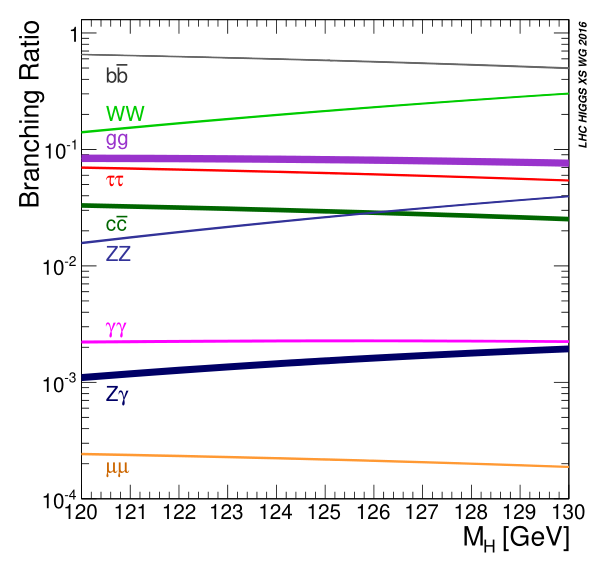
\includegraphics[width=0.5\textwidth]{figures/pheno/higgsBr.png}
\caption{}
\label{fig:higgsBr}
\end{figure}

The partial width of the Higgs boson decaying to two fermions is given by Equation \ref{eqn:higgsDecayFermions}.
\begin{equation}\begin{split}\label{eqn:higgsDecayFermions}
\Gamma(H\to ff)=\frac{G_Fm_f^2m_HN_c}{4\pi\sqrt{2}}(1-4\frac{m_f^2}{m_H^2})^{3/2}
\end{split}\end{equation} 
Here, the $N_c=1$ for leptons (and 3 for quarks) and $G_F=1.166\times10^{-5}$~GeV$^{-2}$ is the Fermi coupling constant.
The total width, $\Gamma$, is defined as the number of decays per time, per particles present.
It is the sum of all partial widths such as the fermionic width in Equation \ref{eqn:higgsDecayFermions}.
The total width is equivalent to the reciprocal \emph{lifetime} of the particle $\tau$, which subsequently defines the particle's half-life as $\tau\ln2$.
The partial width also dictates the \emph{branching ratio} that describes the fraction of decays to a particular final state.
For \hmm decays, the branching ratio is therefore

\begin{equation}\begin{split}
    \text{BR}(\hmm)=\frac{\Gamma(\hmm)}{\Gamma}.
\end{split}\end{equation} 

This equation illuminates the central challenge when studying \hmm. 
The total width of the Higgs is expected to be $4$~MeV and has been measured as $\Gamma=3.2^{+2.8}_{-2.2}$~MeV. \cite{cmsWidth}
The quadratic dependence on the muon mass $m_f=m_\mu$ in the partial width $\Gamma(\hmm)$ leads to a very small branching ratio in the case of the light muon, given in Table \ref{tab:decayCrossSec}.
The partial widths also depend on \mh. This is illustrated in Figure \ref{fig:higgsBr} for the branching ratios including and larger than \hmm.

Experimentally, Higgs production and decay to two muons manifests itself in the dimuon invariant-mass spectrum as a resonance above a smoothly falling background.
The width of the resonance is determined by the total width $\Gamma$, by making use of the uncertainty principle in natural units.
A free particle of mass $m$ with some likelihood to decay to a lower energy state can be described by a simple time dependant wave function,
\begin{equation}\begin{split}
    \psi(t)=\psi(0)e^{-imt}e^{-\frac{\Gamma}{2}t}.
\end{split}\end{equation} 
Here, the first exponential represents the time evolution of a stable particle, while the second represents the decreasing probability that the particle has not decayed.
The $\Gamma$ is the decay rate and also inverse of the exponential time constant.
The fourier transform of the wave equation describes the particle in energy space,
\begin{equation}\begin{split}
    \psi(E)=\int\psi(t)e^{iEt}dt\propto \frac{1}{(E-m)-i\Gamma/2}.
\end{split}\end{equation}
The energy dependant cross section to observe a decay is proportional to $|\psi(E)|^2$, or 
\begin{equation}\begin{split}\label{eqn:breitWigner}
    \sigma(E)\propto\frac{1}{(E-m)^2+\Gamma^2/4}.
\end{split}\end{equation} 
Equation \ref{eqn:breitWigner} gives the relativistic Breit-Wigner function, which describes resonant features in energy spectra.
The width of the resonance corresponds to the decay rate, therefore particles with long lifetimes $\tau$ produce narrow resonances.

The phenomenology of \hmm is determined by these principles.
The Higgs boson decays with a width $\Gamma$ and probability distribution of energies described by the Breit-Wigner function.
In \hmm decays, this energy is converted into the invariant-mass of the dimuon pair, and results in a narrow resonance in the dimuon invariant mass spectrum.
In practice, the energy and momentum resolutions of ATLAS are insufficient to resolve the $\approx4$~MeV width of the Breit-Wigner shape.
Instead a distribution described approximately a Gaussian function with a width corresponding to the invariant-mass resolution is observed.

% VH leptonic
The final state \W or \Z in a VH event offers an opportunity to help identify Higgs events in the same way that the jets in VBF are useful.
This is particularly true when the \W or \Z decays leptonically since these additional leptons offer a clean signal to help remove background.
In the case of \W decays to $\ell^\pm\nu_\ell$ represent $\approx11\%$ of decays for each lepton flavor.
Equation \ref{eqn:wDecayFermions} gives the partial width for leptonic \W decays.
\begin{equation}\begin{split}\label{eqn:wDecayFermions}
    \Gamma(W\to\ell\overline{\nu})=\frac{\sqrt{2}G_Fm_W^3}{12\pi}
\end{split}\end{equation} 
The total width of the \W boson is $\Gamma=2.085\pm0.042$~GeV.
The leptonic branching fraction is smaller in the case of \Z.
The partial width for \Z decays to fermions is given in Equation \ref{eqn:zDecayFermions}.
\begin{equation}\begin{split}\label{eqn:zDecayFermions}
    \Gamma(Z\to f\fbar)=N_c\frac{\sqrt{2}G_Fm_Z^3}{6\pi}\times[(T_3-Q_f\sin^2\theta_W)^2+(Q_f\sin^2\theta_W)^2]
\end{split}\end{equation} 
The total width of the \Z boson is $\Gamma=2.495\pm0.002$~GeV, and the leptonic width is $\Gamma(\Z\to\ll)=83.984\pm0.086$~MeV per lepton flavor.
The result is a leptonic branching ratio of 3.4\% per flavor. \cite{pdg2018}
The measured values of these branching fractions are given in Table \ref{tab:decayCrossSec}.

\section{Contact Interactions and Compositeness}

Contact interactions are a phenomenological description of new physics interactions above the energy scale accessible directly in collisions.
Such interactions lead to increases in the event rate of high mass events in the dilepton invariant invariant-mass spectra. 
A broad assortment of models predict such excesses, but of particular interest are models of composite quarks and leptons.
Even within the space of compositeness models, there is great diversity and no consensus as to the plausibility of a single model. 
As such, it is beneficial to consider the predictions in common with all compositeness models rather than a particular model.
The putative components of fermions are called \emph{preons}, and they are expected to interact through a new strong gauge interaction called \emph{metacolor}.
As is the case of the strong force, metacolor would be infrared confining and asymptotically free.
Below a characteristic energy scale \lam, the interaction binds preons together metacolor singlets observed as quarks and leptons.
While \lam remains unknown, it is clear that it exceeds the fermion masses.
The fermions remain massless relative to \lam through 't Hooft's mechanism. \cite{Eichten:1984eu}
{\color{red} The explanation is in \emph{Recent Developments in Gauge Theories} for 83 euros!}
Early theoretical limits were set by Bhabha-scattering measurements that exclude \lam below 1-2~TeV for electrons. \cite{Eichten:1984eu}
\footnote{Flavor-changing contact interactions are highly constrained through experiment, with limits on \lam excluding values up to hundreds or thousands of TeV.\cite{Eichten:1984eu}}

The particular interest of this thesis is in flavor-diagonal contact interactions.
These models allow either one or both of the fermion's chiral components (\fl and \fr) to be composite.
The presence of parity violating in the standard model motivates the treatment of \fl and \fr as distinct species.
This leads to the general parity violating Lagrangian in Equation \ref{eqn:compLagrangian} which describes a general contact interaction.
\begin{equation}\label{eqn:compLagrangian}
\begin{array}{r@{\,}c@{}c@{\,}l@{\,}l}
\mathcal L = \frac{g^2}{2\Lambda^2}\;[ && \eta_{\mathrm{LL}}&\, (\ufl\gamma_{\mu} \fl)\,(\uflp\gamma^{\mu}\flp) \nonumber \\
& +&\eta_{\mathrm{RR}}& (\ufr\gamma_{\mu} \fr) \,(\ufrp\gamma^{\mu}\frp) \\
&+&\eta_{\mathrm{LR}}& (\ufl\gamma_{\mu} \fl) \,(\ufrp\gamma^{\mu}\frp) \\
&+&\eta_{\mathrm{RL}}& (\ufr\gamma_{\mu} \fr) \,(\uflp\gamma^{\mu}\flp)& ] \: ,\nonumber
\end{array}
\end{equation}
Here $\eta_{ij}$ for $i,j\in\{L,R\}$ are parameters dictating which species are composite: $|\eta_{LL}|=1$ describes composite left-handed fermions, while $|\eta_{LR}|=1$ indicates both \fr and \fl are composite and share common constituents.
In the form given here, a distinction is made between the initial state fermion species ($f$) and final state species ($f'$) because the present interest is in \llqq contact interactions.
This contact interaction Lagrangian describes an approximation of fermion compositeness in the $\shat\llt\lam$ regime.

\begin{figure}[h!]
\captionsetup[subfigure]{position=b}
\centering
\subfloat[][]{{
\feynmandiagram [medium,baseline=(v.base),horizontal=v to b] {
i1 [particle=\(q\)] -- [fermion] v -- [fermion] i2 [particle=\(\qbar\)],
v -- [photon, edge label=\(\gamma^*/Z\)] b,
f1 [particle=\(\ell^{+}\)] -- [fermion] b -- [fermion] f2 [particle=\(\ell^{-}\)],
};
}}
\subfloat[][]{{
\feynmandiagram [medium,baseline=(v.base),horizontal=a to c] {
a[particle=\(q\)] --[fermion] v[blob,label=\(\lam\)] --[fermion] b[particle=\(\qbar\)],
c[particle=\(\ell^{+}\)] --[fermion] v --[fermion] d[particle=\(\ell^{-}\)],
};
}}
\caption{Feynman diagrams representing (a) Drell-Yan, which dominates the standard model contribution to high invariant-mass dilepton production, and (b) a contact interaction of energy scale \lam corresponding to one of the composite models described in Equation \ref{eqn:compLagrangian}.}
\label{fig:ciPheno}
\end{figure}

Contact interactions necessarily modify cross sections of fermion elastic scattering, such as the $q\qbar$ collisions at the LHC.
In the SM the gauge coupling $\alpha_f$ controls high-mass processes through Drell-Yan production.
In their seminal work of 1983, Eichten, Lane, and Peskin showed that if $\alpha_f\llt1$, then the Lagrangian in Equation \ref{eqn:compLagrangian} produces interference of the order $\shat/\alpha_f\lam^2$ with the standard model processes. \cite{eichten}
The diagrams for the dominant standard model process, and a generic contact interaction are shown in Figure \ref{fig:ciPheno}.
The blob in the diagram for the contact interaction emphasizes the generality of Equation \ref{eqn:compLagrangian}. A particular physics model may replace this blob with, for example, an s-channel diagram mediated by the bound state of two prions.
Two possible diagrams to replace the blob are given, for illustrative purpose, in Figure \ref{fig:ciBlobs}.

Since these interactions depend on $q\qbar$ initial states, the relevant parton luminosities that determine the event rates are those of $u\ubar$ and $d\dbar$.
Unfortunately, as illustrated in Figure \ref{fig:partDistFunc}, proton PDFs for $\ubar$ and $\dbar$ are relatively small since these are produced as virtual sea quarks.
This suppresses the production of $q\qbar$ initial states, and consequently of this type of contact interaction.
If the LHC had been designed to use $p\pbar$ collisions of equal intensity, it would greatly enhance the $q\qbar$ luminosities.

\begin{figure}[h!]
\captionsetup[subfigure]{position=b}
\centering
\subfloat[][]{{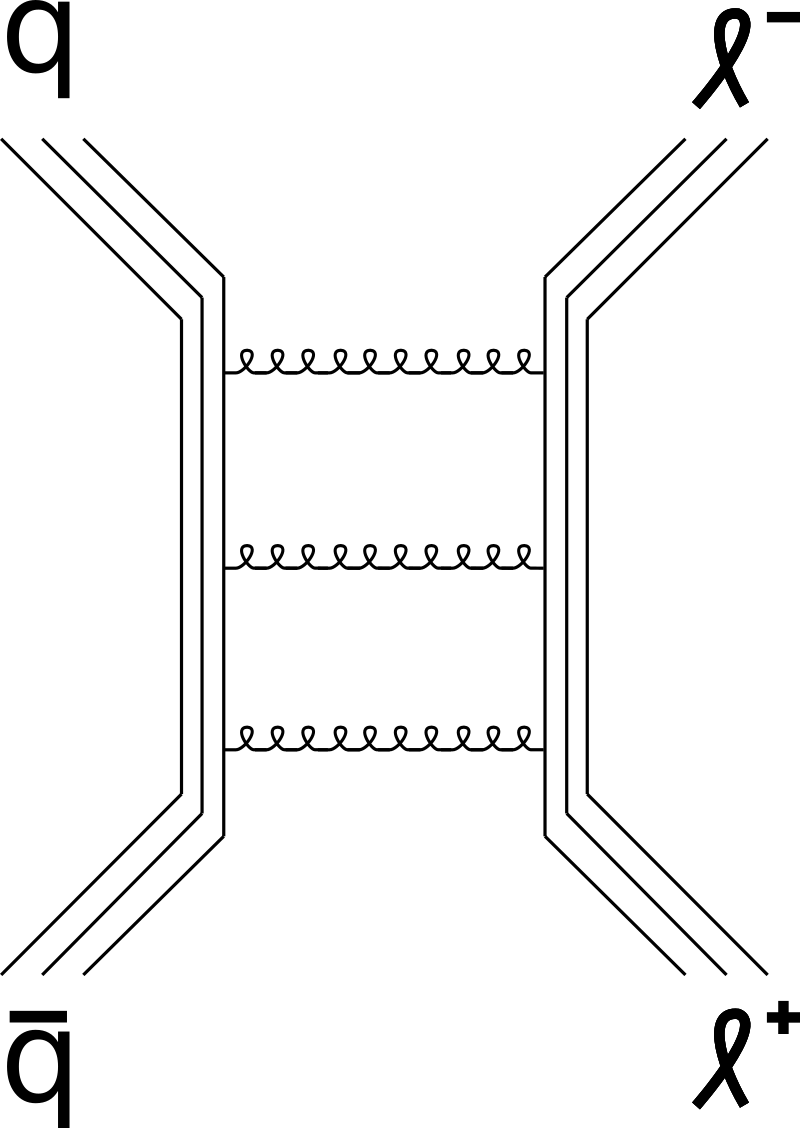
\includegraphics[height=0.20\textheight]{figures/pheno/ciGluon.png}}}
\hspace{0.15\textwidth}%
\subfloat[][]{{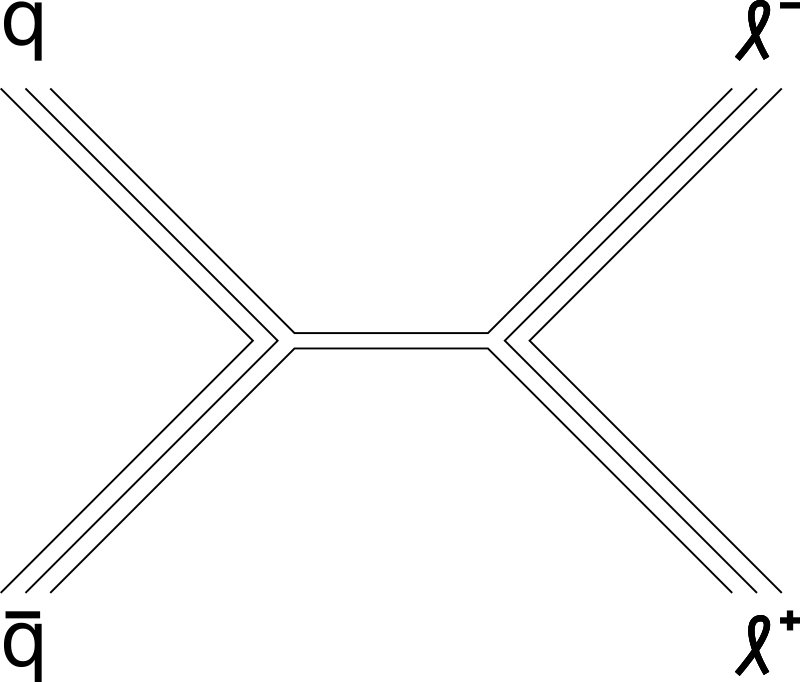
\includegraphics[height=0.20\textheight]{figures/pheno/ciSchan.png}}}
\caption{Feynman diagrams for two possible high-energy processes that may result from fermion compositeness. The solid lines represent the preons composing the fermions. In subfigure (a), an interaction mediated by the bound state of two prions, which is only possible when the leptons and quarks share common constituents. In subfigure (b), an interaction between quarks and leptons mediated by ``metacolor gluon'' exchange, represented by curly lines in analogy to SU(3) gluons.{\color{red} Find way to make better diagrams}}
\label{fig:ciBlobs}
\end{figure}

%%% Specific ll-qq CI $$$
This thesis focuses on \llqq contact interactions, which are a subset of those described by Equation \ref{eqn:compLagrangian}.
Such models replace the unprimed $f$ with quarks, and the primed $f'$ with leptons.
This interaction is possible if the quarks and leptons share common constituents, in which case interactions mediated by the constituents are possible as shown in Figure \ref{fig:ciBlobs} (a).
This interaction is also possible if the fermions do not share common constituents as shown in Figure \ref{fig:ciBlobs} (b).

The Drell-Yan differential cross section is modified in the case of left-left compositeness, $\eta_{LL}=\pm1$ and $\eta_{LR}=\eta_{RL}=\eta_{RR}=0$.

\begin{flalign}\label{eqn:}
\frac{d\hat{\sigma}}{d\that}(q_i\qbar_i\to\ll) =& \frac{\pi\alpha^2}{\shat^2}\left[A_i(\shat)\left(frac{\uhat}{\shat}\right)^2+B_i(\shat)\left(frac{\that}{\shat}\right)^2\right] \notag\\
\end{flalign} 
Here, the coefficients are defined as functions of \shat.
\begin{flalign}\label{eqn:}
A_i(\shat) =& \left[Q_i-\frac{L_iL_l}{4x_W(1-x_w)}\frac{\shat}{\shat-M_Z^2+iM_Z\Gamma_Z}-\frac{\eta_{LL}\shat}{\alpha\lam^2}\right]^2 + \notag\\
            & \left[Q_i-\frac{R_iR_l}{4x_W(1-x_w)}\frac{\shat}{\shat-M_Z^2+iM_Z\Gamma_Z}\right]^2  \notag\\
B_i(\shat) =& \left[Q_i-\frac{R_iL_l}{4x_W(1-x_w)}\frac{\shat}{\shat-M_Z^2+iM_Z\Gamma_Z}\right]^2 + \notag\\
            & \left[Q_i-\frac{L_iR_l}{4x_W(1-x_w)}\frac{\shat}{\shat-M_Z^2+iM_Z\Gamma_Z}\right]^2  \notag\\
\end{flalign}
In these equations, $i,j\in\{u,d\}$ stand for quark flavors.
As was defined when discussing Higgs production in Section \ref{sec:phenoHiggs}, $L_i=T_3-2Q_ix_W$, $R_i=-2Q_ix_W$, and $x_W=\sin^2\theta_W$. {\color{red} coordinate notation}
$Q_i$ is the electric charge of the corresponding quark flavor. \cite{Eichten:1984eu} % supercollider

Despite their verbosity, these equations readily illuminate the phenomenology relevant to the contact interaction search.
First, when setting $\eta_{LL}=0$, the standard model Drell-Yan production is recovered.
Expanding the first power term in $A_i(\shat)$ yields a \emph{direct} term that contributes to the total cross section and scales as $\lam^{-4}$.
Removing the \lam defines the contact interaction form factor $F_C$,
\begin{equation}\begin{split}
    % \Delta\left[\frac{d\hat{\sigma}}{d\that}\right] = \frac{\pi\alpha^2}{\shat^2}\left[\frac{\shat}{\alpha^2}\left(\frac{\uhat}{\shat}\right)^2 \right] /\lam^4
    F_C(\shat) \equiv \frac{\pi\uhat^2}{\shat^2}.
\end{split}\end{equation} 
{\color{red} Check d\that vs d\mll}
Since $F_C$ is strictly positive, it enhances the total \qqll cross section regardless of the sign of $\eta_{LL}$.
The cross terms in the expansion dictate the interference of the contact interaction with Drell-Yan.
Again removing the \lam factor defines the interference form factor $F_I$,
\begin{equation}\begin{split}
    F_I(\shat) \equiv -2\eta_{LL}\left[Q_i-\frac{L_iL_l}{4x_W(1-x_w)}\frac{\shat}{\shat-M_Z^2+iM_Z\Gamma_Z}\right]\frac{\pi\alpha\uhat^2}{\shat^3}.
\end{split}\end{equation} 
The sign of $F_I$ depends on the sign of $\eta_{LL}$.
For $\eta_{LL}=-1$, $F_I$ contributes constructively to the total cross section, while for $\eta_{LL}=+1$ it leads to destructive interference that reduces the overall cross section.

Together, $F_I$ and $F_C$ describe the effect of contact interactions as functions of collision energy, without making reference to the particular manifestation of fermion compositeness.
The functional dependence on \shat leads to the expression of the interference form factor $F_I$ at relatively low energies compared to the direct form factor $F_C$.
Experimentally this results in interference effects altering dilepton spectra at lower invariant-mass, and direct production always enhancing the spectra in the high mass tail.
These effects are broad in the invariant-mass spectra, as opposed to the narrow resonance expected from \hmm production.
The modification to the total cross section has the form,
\begin{equation}\label{eqn:cixsPheno}
\frac{\text{d}\sigma}{\text{d}m_{\ell\ell}} = \frac{\text{d}\sigma_\textrm{DY}}{\text{d}m_{\ell\ell}} - \eta_{ij}\frac{F_\textrm{I}}{\Lambda^2} + \frac{F_\textrm{C}}{\Lambda^4}.
\end{equation}

Although various compositeness models predict variations on these results, there are two points to consider.
First, the functional dependence on the energy \shat is common for all contact interactions. \cite{Eichten:1984eu}.
Second, the modification to the effect on the total cross section is substantially of the same magnitude regardless of the form of compositeness.
Combined, these make the described formalism an attractive framework to study compositeness without reference to the particular model.


% \cite{acosta} % LHC prospect
